\chapter{Theory}
\lhead{\emph{Theory}}
% TODO CITE
% KERAS
% SKLEARN
% NUMPY


\section{Handwriting recognition}
% history
% on-line and off-line
% 
Handwriting recognition systems are computer systems that can recognize characters and symbols written by hand. These systems have been continuously developed and researched ever since the ancient days of computers \parencite{simon_off-line_1992}, beginning with the optical character recognition (OCR) systems in the 1950s \parencite{mori_historical_1992}. The early OCR systems were very limited in terms of hardware, which resulted in a great deal of testing and failing. Researchers had high aspirations for handwriting recognition, but progress was slow and it gained the reputation of being an extremely difficult problem \parencite{simon_off-line_1992}. As hardware and computers became more advanced, the OCR and handwriting recognition systems followed in the same direction. Hardware has usually been the bottleneck for these systems (trenger kilde).

When computational power increased, using artificial neural networks became more popular, also for handwriting recognition. For example, in (TODO kilde fukushima, wake), a neural network was trained to recognize 35 symbols. Since then, neural networks has been used in many solutions, and has proven to be a major contributor to the field, as it is one of the most used tools in the leading solutions today (some of these are presented in section \ref{recognition of handwritten mathematics}).

This field has for a long time been a worldwide research project \parencite{mori_historical_1992}. Many competitions on different handwriting recognition problems has been arranged, and researchers from all over the world has cooperated to produce solutions This further confirms the difficulty of a general handwriting recognition system. 

\subsection{Main approaches}

Handwriting recognition systems generally has two main approaches, online and offline \parencite{priya_online_2016}. Online recognition uses data from pen strokes based on sampled coordinates of pen movements and the time difference between them. These pen strokes are also referred to as traces and is stored separately. This means that strokes can easily be separated, which in many ways can aid in the segmentation problem (see section \ref{the_segmentation_problem}).

While online recognition uses dynamic data, offline recognition uses static data such as images. In this approach the recognition system has to rely solely on pixel values in the images, which introduces some complications. For instance, these systems can't separate traces in the same easy way as online recognition systems since only images are available. 

\begin{figure}[H]
\centering
\begin{subfigure}{0.3\textwidth}
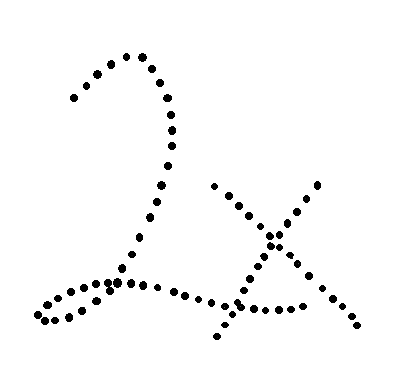
\includegraphics[width=1.1\linewidth, height=5cm]{Assets/Chapter2_Theory/segmentation_2_on.png} 
\caption{}
\label{fig:online_data}
\end{subfigure}
\begin{subfigure}{0.3\textwidth}
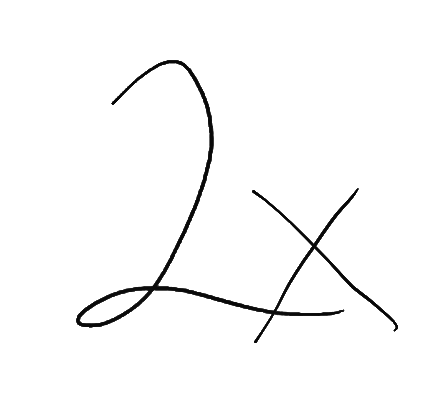
\includegraphics[width=1.1\linewidth, height=5cm]{Assets/Chapter2_Theory/segmentation_2.png}
\caption{}
\label{fig:offline_data}
\end{subfigure}
\caption{A: Online recognition data with coordinate samples. B: Offline recognition data (only an image).}
\label{fig:online_offline_comparison}
\end{figure}

With the online input data, there is possible to create an image of all the traces by drawing a line between the coordinates. This means that online recognition systems has access to the same images as offline recognition systems, as well as coordinates for each of the traces. Having more accurate input data and more features to analyze is important since handwriting is different from person to person. In general, online recognition systems has higher performance than offline recognition systems \parencite{priya_online_2016}.

\subsection{Common steps in handwriting recognition}

In the recognition process there are several problems that must be solved. Usually, the most common problems include segmentation and classification of symbols. In addition, the pre- and post-processing steps can be heavy and demanding.

\subsubsection{Pre-processing}

In the pre-processing step the raw input data is prepared for analysis. Raw input data can come in many formats and sizes. In addition, the input data may contain values that are not valid. This step deals with these problems by converting the data to a format that suits the consecutive steps better.

A common task in pre-processing is to normalize the input data. This simply means that all the data is scaled to the same value range. 


For handwriting recognition pre-processing can be a heavy step. 

\subsubsection{The segmentation problem} \label{the_segmentation_problem}

The segmentation problem deals with segmenting symbols from traces. 

\begin{figure}[H]
\centering
\begin{tikzpicture}
\begin{scope}[xshift=1.5cm]
    \node[anchor=south west,inner sep=0] (image) at (0,0) {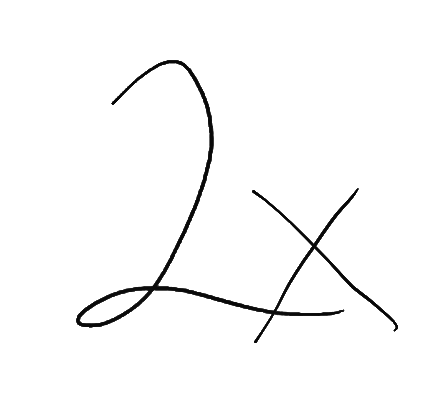
\includegraphics[width=0.2\textwidth]{Assets/Chapter2_Theory/segmentation_2.png}};
    \begin{scope}[x={(image.south east)},y={(image.north west)}]
        \draw[->] (1,0.5) -- (1.9,0.8);
        \draw[->] (1,0.4) -- (1.9,0.4);
        \draw[->] (1,0.3) -- (1.9,0);
        \node [anchor=west] (note) at (2,0.9) {\Large 2x};
        \node [anchor=west] (note) at (2,0.4) {\Large $\Delta$};
        \node [anchor=west] (note) at (2,-0.1) {\Large 2/\textbackslash};
        \node [anchor=west] (note) at (2.4,0.4) {\Huge ?};
    \end{scope}
\end{scope}
\end{tikzpicture}
\caption{The segmentation problem deals with segmenting symbols from traces. The sample above has three traces, one for the "2"  and two for the "x". Correctly segmenting the symbols is a difficult problem since traces can overlap in countless ways.}
\label{fig:segmentation}
\end{figure}

\subsubsection{Classification of symbols}
% classifiers
% Neural nets
% 

\subsubsection{Post-processing}
% Interpretation, based on truths
Presentation of classification result

Further interpretation analysis

Contextual analysis

Correcting errors done by the classifier

\subsection{Recognition of handwritten mathematics} \label{recognition of handwritten mathematics}
% Problem more specific to our case
% context/interpretation after classifying
% Existing solutions

Recognition of handwritten mathematics is a field in handwriting recognition that deals with mathematical symbols and expressions. This field has many of the same problems as recognition of words and characters, however, there is also a new problem that must be dealt with. Just as regular language, mathematics has a set of grammatical or positional rules that should be followed. However, this is not the same type of grammar. For example, there are fractions, exponents and square root that must be interpreted based on positional values. A context of how all the symbols fit together has to be built.


% Illustration of the recognition process
\begin{figure}[H]
  \centering
\end{figure}




\subsection{Previous work and existing solutions}
% thesis from 1999
% mathpix
% Myscript
% chromhe 
Many have tried to create systems for recognition of handwritten mathematics. 



\subsection{InkML}
InkML is a markup language based on XML to describe digital ink data. The format is specified by the World Wide Web Consortium (W3C) \cite{chee_ink_2011}. InkML groups it's content in specific XML-style elements called ink, the ink element often has sub elements which is a trace element.\\

\begin{minipage}{\linewidth}
\begin{lstlisting}[language=XML, %
label={lst:InkML_ex},
caption={\textbf{\gls{InkML}} example of three traces, each with an file-unique id. In addition to traces, we have listed a tracegroup, which specifies what and where the traces belong to. Truths are used when providing labels to use in supervised learning, which is explained later in this chapter.}]
<trace id="0">
    207 136, 199 141, 197 143, 196 144, 195 146, 194 147, 193 149
</trace>
<trace id="1">
    847 201, 847 204, 846 207, 846 211, 846 215, 845 219, 845 222
</trace>
<trace id="2">
    833 235, 822 235, 821 235, 820 235, 819 236, 819 235, 819 236
</trace>

<traceGroup xml:id="3">
	<annotation type="truth">+</annotation>
	<traceView traceDataRef="1"/>
	<traceView traceDataRef="2"/>
	<annotationXML href="+_1"/>
</traceGroup>
\end{lstlisting}
\end{minipage}


\section{\LaTeX}
% Talk about it from a historical perspective
% Talk about how CROHME have advanced the art of recognizing handwritten math.
% Talk about how it can be used

% Talk about 
\LaTeX is a tool for preparing documents for high-quality typesetting. It is most regularly used in the creation of technical or scientific documents, but it is versatile. Thus, it's useful in almost any type of publishing.\parencite{_introduction_2018} \\ % tynn suppe, men vanskelig å finne mer



\section{Machine learning}
% 2.3 gjennomgang 18.04.2018
% Bruk en mer relevant aktør enn youtube
% 

We are currently living in a time where big data surrounds us in our daily lives. Take YouTube for example, YouTube has over one billion users, each day several hundred millions of hours are being watched and every second 5 hours of YouTube content is uploaded. \\ % CITE YOUTUBE press stats og FORTUNE LORD [Ikke god nok kilde?]
 This massive ammount of data could benefit from analysis, which is what machine learning is doing. According to \cite{murphy_machine_2012}, machine learning can be defined as a set of methods that can automatically detect patterns in data. These uncovered patterns can also be used to predict future data or support decision making. For example, in \cite{cline_predictive_2017}, historical data of maintenance is used to predict failure for individual mechanical parts. \\
\cite{goodfellow_deep_2016} explains machine learning as an applied form of statistics, which uses computers to do statistic estimations on complicated functions and decreased attention on proving the related confidence intervals. 


% Introduce ML, training machines to learn patterns, pattern recognition, Short explanation, Examples, pros cons
\subsection{Supervised learning}
% Anmeldelse 18.04.2018
% 

Supervised learning is the machine learning task to map an input to an output. The training data needed has features in addition to a label. For example, to train a model(in this case, a neural network) in the case of supervised learning, one would need to supply the model with a lot of training data, in addition to labels associated with the data. %In this projects case the InkML data contains both sequential coordinates and a label. See InkML example \ref{lst:InkML_ex}. In the InkML data, our labels are the truth associated with each trace or tracegroup.\\

If you want to classify or use any supervised learning algorithm, the algorithm could study many examples of what it's going to classify to eventually be able to classify to the correct class, which in this case is labels associated with mathematical symbols.\\ To explain this in another way think of the function p(y $|$ x), this reads the probability of y given x has happened. This is exactly what supervised learning is, the y labels are provided by a supervisor.\\

%\subsection{Unsupervised learning} is this needed?
On the other hand we have unsupervised learning which is basically observation and after observing data it attempts to learn probability distribution p(x) of them implicit or explicit. An example of unsupervised learning is clustering. In clustering the goal is to divide the data into different clusters based on their attributes. \parencite{goodfellow_deep_2016}
% veldig kort om unsupervised, vi går ikke i detaljer. 

\section{Artificial neural networks}

Artificial neural networks are 
% Introduce
% Inspired by biological neural networks
% The goal is to approximate some function
% 
% 

\subsection{Core concepts}
% Briefly introduce the core concepts for understanding ANN's

%\subsubsection{Components in a neural network}
% Neurons
% briefly explain how layers are connected to each other, how weights changes
% illustrations!

A neural network consists of a combination of artificial neurons, also referred to as computational units. These neurons takes a vector as input. The input is multiplied the with precomputed weights, and a bias is added. Then the result is summed and used as input to the activation function (\ref{activation_functions}). Lastly the weighted sum is returned as output from the neuron. \parencite{_cs231n_????} \parencite{_multi-layer_????}



\begin{figure}[H]
  \centering
    \begin{tikzpicture}
        \draw[->] (0,2) -- (2.1,0.8);
        \draw[->] (0,0.65) -- (2,0.3);
        \draw[->] (0,-0.65) -- (2,-0.3);
        \draw[->] (0,-2) -- (2.1,-0.8);
    
        \node at (0.2, 2.3) {$x_1$};
        \node at (0.2, 1) {$x_2$};
        \node at (0.2, -0.25) {$...$};
        \node at (0.2, -1.5) {$x_n$};
        
        \draw [] (4.2,0) ellipse (2cm and 1cm);
        
        \node at (4.2,0) {$\sum\limits_{i=1}^{n} W_i \cdot x_i + b$};
        
        \draw[->] (6.5,0) -- (7.5,0);
        
        \draw (7.8, 0.8) rectangle (9.8, -0.8);
    
        \node at (8.8,0) {$f : R \rightarrow R$};
    
    \end{tikzpicture}
    \caption{Diagram of a single artificial neuron.} % TODO denne trenger mer kjøtt, god forklaring fra a til å!
    \label{fig:single_neuron}

\end{figure}

The neurons in a neural network are typically organized into different layers, where each layer has a fixed number of neurons. The diagram below is an example of how these neurons can be connected together.

\begin{figure}[H]
  \centering

    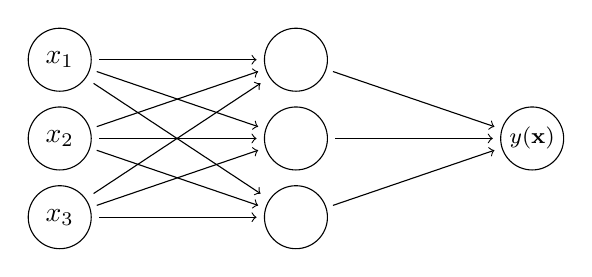
\begin{tikzpicture}
        
        \draw [] (0.5,1) circle [radius=0.4];
        \draw [] (0.5,0) circle [radius=0.4];
        \draw [] (0.5,-1) circle [radius=0.4];

        \draw [] (3.5,1) circle [radius=0.4];
        \draw [] (3.5,0) circle [radius=0.4];
        \draw [] (3.5,-1) circle [radius=0.4];

        \draw [] (6.5, 0) circle [radius=0.4];

        \draw[->] (1,1) -- (3,1);
        \draw[->] (0.97,0.85) -- (3.02,0.15);
        \draw[->] (0.93,0.7) -- (3.05,-0.7);

        \draw[->] (0.97,0.15) -- (3.02,0.85);
        \draw[->] (1,0) -- (3,0);
        \draw[->] (0.97,-0.15) -- (3.02,-0.85);

        \draw[->] (0.93,-0.7) -- (3.05,0.7);
        \draw[->] (0.97,-0.85) -- (3.02,-0.15);
        \draw[->] (1,-1) -- (3,-1);
        
        \draw[->] (3.97,0.85) -- (6.02,0.15);
        \draw[->] (4, 0) -- (6,0);
        \draw[->] (3.97, -0.85) -- (6.02,-0.15);

        \node at (0.5,1) {$x_1$};
        \node at (0.5,0) {$x_2$};
        \node at (0.5,-1) {$x_3$};
        \node at (6.5,0) {\footnotesize$y(\textbf{x})$};

    \end{tikzpicture}
    \caption{Diagram of a single layered neural network. It contains three neurons in the input layer, three neurons in the hidden layer, and a single neuron in the output layer. }
    \label{fig:single_layered_neural_network}
\end{figure}


The leftmost \textbf{\gls{layer}} of neurons in \ref{fig:single_layered_neural_network} is called the input layer. The input layer is a passive layer, meaning the layer does not modifiy the data. Each neuron in the input layer receives a single input and duplicate the input to its multiple output neurons. The hidden layer and the output layer from \ref{fig:single_layered_neural_network} are active neurons. These neurons modify the data before propagating the values to the next layer. The modifications are described in \ref{fig:single_neuron}. The result of the output layer is the approximation done by the neural network. \parencite{smith_scientist_1997} 
In order for a neural network to be a good approximator, the weights and biases in each neuron has to be optimized to minimize error in the output layer. This tuning process is performed through training. Training a network means giving the network labeled training data, comparing the output label from the network to the label provided, and tuning the weights and biases to best satisfy a loss function (\ref{loss_function}). This optimization process is typically done using an optimizer such as gradient decent, and through a concept called backpropogation. This is described in detail in \ref{training_with_backpropagation}.
%\subsubsection{Layers}
% Dense
% Deep neural networks
% 

\subsection{Activation functions}
\label{activation_functions}

% math formulas

Activation functions in artificial neural networks has inspiration from how neurons in our brain works. In a mathematical model of an artificial neuron by McCulloch-Pitt \cite{mcculloch_logical_1943}, the activation of a neuron was modelled as the unit step function. This model has later been generalized to use functions such as sigmoid, rectified linear unit, softmax and tangens hyperbolicus. \parencite{jain_artificial_1996}

\begin{figure}[H]
  \centering
    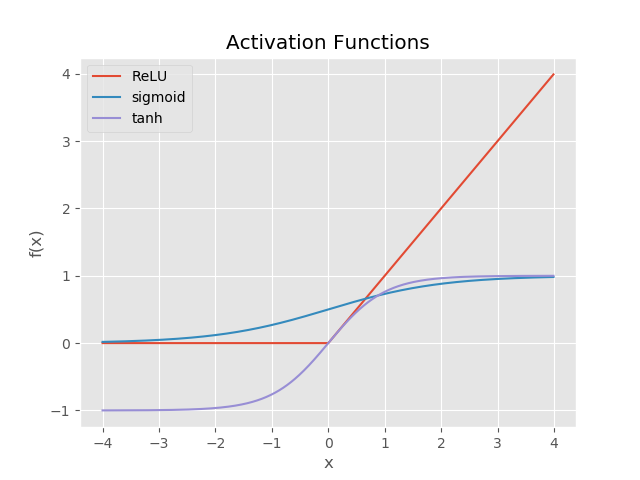
\includegraphics[width=0.9\textwidth]{Assets/Chapter2_Theory/activation_function_overview.png}
    \caption{Three activation functions plotted on the interval [-4,4].}
\end{figure}

One purpose of an activation function is to introduce nonlinearity into the model. A network without nonlinearity can not represent functions which are nonlinear, despite having multiple layers. On the other hand, it is proved that. \cite{leshno1993multilayer}

\begin{quote}
A standard multilayer feedforward network with a locally bounded piecewise
continuous activation function can approximate any continuous function to any degree of
accuracy if and only if the network's activation function is not a polynomial.
\end{quote}
 An example of the importance of nonlinearity in neural networks can shown in the exclusive-OR problem. \parencite{jain_artificial_1996}\cite{sharma_understanding_2018}

\begin{figure}[H]
  \centering

    \begin{subfigure}{.45\textwidth}
      \centering

        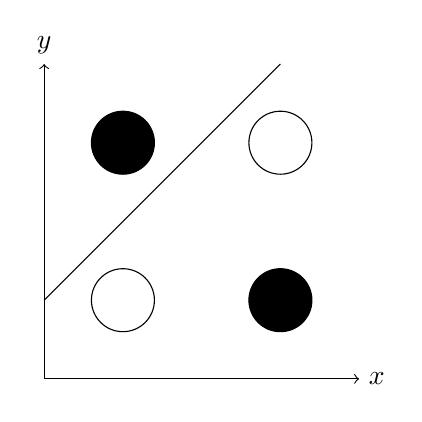
\begin{tikzpicture}
        
            \draw [fill=black] (0.5,1) circle [radius=0.4];
            \draw [] (0.5,-1) circle [radius=0.4];
    
            \draw [] (2.5,1) circle [radius=0.4];
            \draw [fill=black] (2.5,-1) circle [radius=0.4];
    
            \draw[-] (-0.5, -1) -- (2.5,2);
    
            \draw[->] (-0.5,-2) -- (3.5,-2) node[right] {$x$};
            \draw[->] (-0.5,-2) -- (-0.5, 2) node[above] {$y$};

        
        \end{tikzpicture}
        \caption{Using no activation functions}

    \end{subfigure}
    \begin{subfigure}{.45\textwidth}
      \centering

        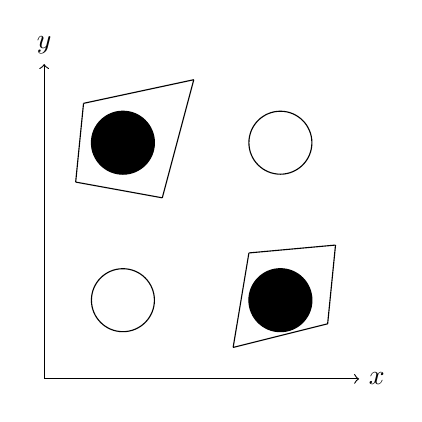
\begin{tikzpicture}
        
            \draw [fill=black] (0.5,1) circle [radius=0.4];
            \draw [] (0.5,-1) circle [radius=0.4];
    
            \draw [] (2.5,1) circle [radius=0.4];
            \draw [fill=black] (2.5,-1) circle [radius=0.4];
    
            \draw[-] (0, 1.5) -- (-0.1,0.5);
            \draw[-] (-0.1, 0.5) -- (1,0.3);
            \draw[-] (1, 0.3) -- (1.4,1.8);
            \draw[-] (1.4, 1.8) -- (0,1.5);
    
            \draw[-] (1.9, -1.6) -- (3.1, -1.3);
            \draw[-] (3.1, -1.3) -- (3.2,-0.3);
            \draw[-] (3.2, -0.3) -- (2.1,-0.4);
            \draw[-] (2.1, -0.4) -- (1.9,-1.6);
    
            
            \draw[->] (-0.5,-2) -- (3.5,-2) node[right] {$x$};
            \draw[->] (-0.5,-2) -- (-0.5, 2) node[above] {$y$};
        \end{tikzpicture}
        \caption{Using non-linear activation functions}
        % TODO verifiser formen på denne? den forrige har linje, men denne har ikke (?)
        % Denne er riktig tegnet, men klassifiseringen må fylles inn, og problemet må forklares bedre

    \end{subfigure}
    
    \caption{Figure of the exclusive-OR problem, by the capabilities of a model with non-linear activation functions versus no activation function.}
    \label{fig:exclusive-OR problem}
\end{figure}

Activation functions are also important for squashing the output of a neural network into desired bounds. A common use case is for returning class probabilities for a classification model, where softmax is often used as the activation function for the last layer. Softmax is an activation function which transforms its inputs to a combined sum of 1.\cite{sharma_understanding_2018}

\begin{figure}[H]
  \centering
    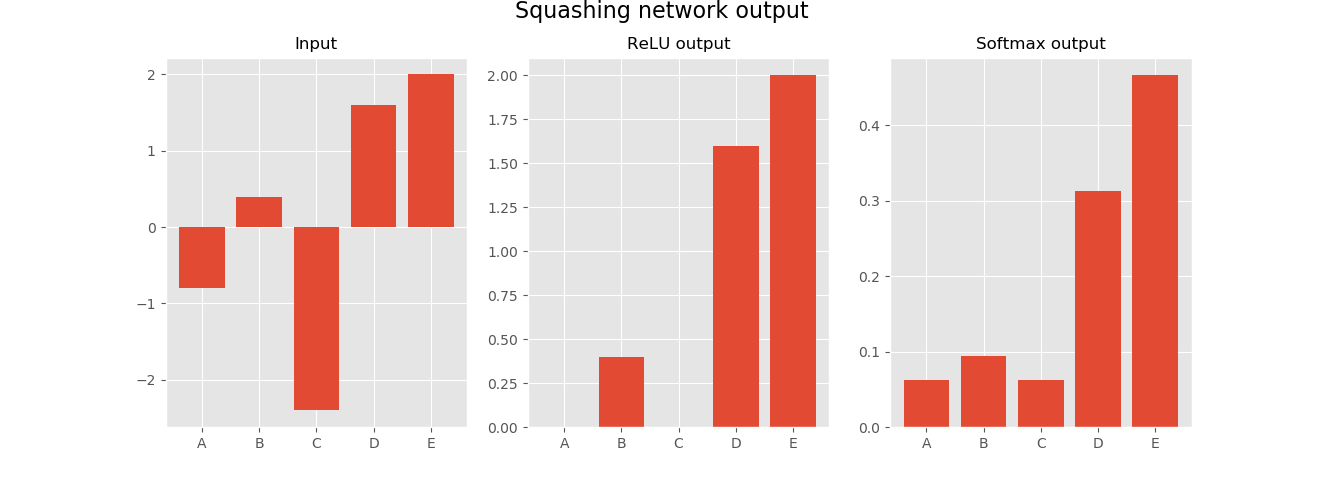
\includegraphics[width=\textwidth]{Assets/Chapter2_Theory/squashin_output_data_using_activation_functions.png}
    \caption{Figure of how example input data is transformed through two different activation functions. Data flows from left to right, with output from last graph used as input to the next.}
\end{figure}




\subsubsection{ReLU}

Rectified linear unit or ReLU is a non-linearity introduced by Hanloser et al. in 2000 \cite{smith_scientist_1997}, and has later been found successful as a nonlinearity in deep neural network. It is a function which disallows negative values, and outputs the input if positive, else it outputs 0.

\begin{equation}
    f(x) = max(x, 0)
\end{equation}

ReLU is a cheap mathematical operation to perform, as the max operation only includes addition, multiplication and comparison, while other previously popular nonlinearities are dependent on calculating exponential functions. 

ReLU has also performed well compared to other nonlinearities in stochastic gradient descent (SGD) \ref{calculating_an_output}. Krizhevsky et al. demonstrated an improvement of a factor of six, when comparing number of epochs needed to reach 25\% error rate with a network using ReLU, compared to an equivalent network with tanh as a nonlinearity. \cite{krizhevsky_imagenet_2012}

A negative side effect from ReLU is the dying ReLU problem, where neurons can be pushed to a state where the neuron will output the same value regardless of input. This is a variation of the vanishing gradient problem \ref{vanishing-gradient}. The concept of dead neurons is described in \ref{dead-neurons}\cite{zeiler_rectified_2013}

\subsubsection{Softmax}

Softmax is an activation which transforms its inputs to a distribution which adds up to one. This makes the softmax function useful to represent probabilities, and is therefor often used on the last layer of neural networks. Combined with the loss function categorical cross entropy \ref{categorical-crossentropy}, softmax can be used to predict multiclass classification. \cite{_cs231n_????-1}
\begin{equation}
    f_j(z) = \frac{e^{z_j}}{\sum_k e^{z_k}}
\end{equation}



\subsubsection{Sigmoid}

Sigmoid has been a historically popular function as activation function. It works by squashing the input to the range $[0, 1]$, where small numbers are returned as a value close to 0, and large numbers are returned as values close to 1. 

\begin{equation}
    \sigma(x) = 1 / (1 + e - x)
\end{equation}

An issue with sigmoid is that the outputs are not zero-centered, which means the output of the function will all be of the same sign. When these values are sent to the next layer of the network, the inputs will cause the gradients to be the same sign as well. This can cause undesirable updates of weights during backpropagation, with zig-zag dynamics for weight updates. \cite{_neural_2018}

\subsubsection{Tanh}

Tanh is an activation function with similar characteristics as sigmoid, and can be represented as a scaled sigmoid (which can be seen in the equation below).

Tanh, however, squashes the inputs to the range $[-1, 1]$, which means it does not inherit the same issues with non zero-centered outputs. Therefore, in practice, tanh is always preferred to sigmoid. \cite{_neural_2018}

\begin{equation}
    tanh(x) = 2 \cdot \sigma(2x) - 1
\end{equation}

\subsection{Calculating an output}
\label{calculating_an_output}

The output of a neural network is generally a list of numerical values. This vector contains as many values as there are output units in the neural network. To create this output vector the neural network performs a series mathematical operations on the input vector. 

For this demonstration the network in figure \ref{fig:single_layered_neural_network} will be used. The first step is to calculate the outputs from the hidden layer, $H_o$ (figure \ref{fig:calculating_output_one}).
\begin{figure}[H]
  \centering

    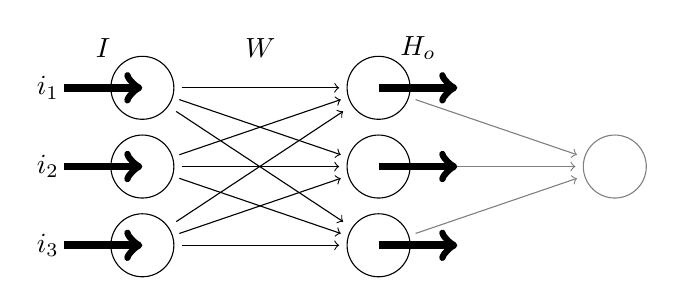
\begin{tikzpicture}
        
        \draw [] (0.5,1) circle [radius=0.4];
        \draw [] (0.5,0) circle [radius=0.4];
        \draw [] (0.5,-1) circle [radius=0.4];

        \draw [] (3.5,1) circle [radius=0.4];
        \draw [] (3.5,0) circle [radius=0.4];
        \draw [] (3.5,-1) circle [radius=0.4];

        \draw [draw={rgb:black,2;white,2}] (6.5, 0) circle [radius=0.4];

        \draw[->] (1,1) -- (3,1);
        \draw[->] (0.97,0.85) -- (3.02,0.15);
        \draw[->] (0.93,0.7) -- (3.05,-0.7);

        \draw[->] (0.97,0.15) -- (3.02,0.85);
        \draw[->] (1,0) -- (3,0);
        \draw[->] (0.97,-0.15) -- (3.02,-0.85);

        \draw[->] (0.93,-0.7) -- (3.05,0.7);
        \draw[->] (0.97,-0.85) -- (3.02,-0.15);
        \draw[->] (1,-1) -- (3,-1);
        
        \draw[draw={rgb:black,2;white,2}, ->] (3.97,0.85) -- (6.02,0.15);
        \draw[draw={rgb:black,2;white,2}, ->] (4, 0) -- (6,0);
        \draw[draw={rgb:black,2;white,2}, ->] (3.97, -0.85) -- (6.02,-0.15);

        %\node at (0.5,1) {$x_1$};
        %\node at (0.5,0) {$x_2$};
        %\node at (0.5,-1) {$x_3$};
        %\node[text={rgb:black,2;white,2}] at (6.5,0) {\footnotesize$y(\textbf{x})$};
        
        \draw[->, line width=1mm] (3.5,1) -- (4.5,1);
        \draw[->, line width=1mm] (3.5,0) -- (4.5,0);
        \draw[->, line width=1mm] (3.5,-1) -- (4.5,-1);
        
        \draw[->, line width=1mm] (-0.5,1) -- (0.5,1);
        \draw[->, line width=1mm] (-0.5,0) -- (0.5,0);
        \draw[->, line width=1mm] (-0.5,-1) -- (0.5,-1);
        
        \node at (0,1.5) {$I$};
        \node at (-0.7,1) {$i_1$};
        \node at (-0.7,0) {$i_2$};
        \node at (-0.7,-1) {$i_3$};
        
        \node at (2,1.5) {$W$};
        \node at (4,1.5) {$H_o$};
        
        

    \end{tikzpicture}
    \caption{}
    \label{fig:calculating_output_one}
\end{figure}

Each of the input values are multiplied with the weight to each unit in the hidden layer. All the inputs to a unit in the hidden layer is then summed. Matrix multiplication can be used for this, where a matrix containing all the weights is multiplied with a column-matrix containing the input values. The weights matrix is a 3x3 matrix since there are 3 inputs and 3 units in the hidden layer.

\begin{center}
$
W * I = 
\begin{bmatrix} 
w_{1,1} & w_{2,1} & w_{3,1}\\
w_{1,2} & w_{2,2} & w_{3,2}\\
w_{1,3} & w_{2,3} & w_{3,3}
\end{bmatrix}
*
\begin{bmatrix} 
i_1\\
i_2\\
i_3
\end{bmatrix}
=
\begin{bmatrix} 
h_1\\
h_2\\
h_3
\end{bmatrix}
=
H_i
$
\end{center}

To calculate the output from the hidden layer the activation function chosen is used on these input values.

\begin{center}
$
activation(H_i) = H_o
$    
\end{center}

The output from the hidden layer is then sent further in the network.

\begin{figure}[H]
  \centering

    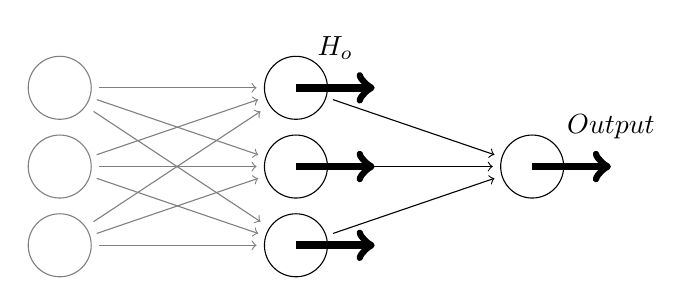
\begin{tikzpicture}
        
        \draw [draw={rgb:black,2;white,2}] (0.5,1) circle [radius=0.4];
        \draw [draw={rgb:black,2;white,2}] (0.5,0) circle [radius=0.4];
        \draw [draw={rgb:black,2;white,2}] (0.5,-1) circle [radius=0.4];

        \draw [] (3.5,1) circle [radius=0.4];
        \draw [] (3.5,0) circle [radius=0.4];
        \draw [] (3.5,-1) circle [radius=0.4];

        \draw [] (6.5, 0) circle [radius=0.4];

        \draw[draw={rgb:black,2;white,2}, ->] (1,1) -- (3,1);
        \draw[draw={rgb:black,2;white,2}, ->] (0.97,0.85) -- (3.02,0.15);
        \draw[draw={rgb:black,2;white,2}, ->] (0.93,0.7) -- (3.05,-0.7);

        \draw[draw={rgb:black,2;white,2}, ->] (0.97,0.15) -- (3.02,0.85);
        \draw[draw={rgb:black,2;white,2}, ->] (1,0) -- (3,0);
        \draw[draw={rgb:black,2;white,2}, ->] (0.97,-0.15) -- (3.02,-0.85);

        \draw[draw={rgb:black,2;white,2}, ->] (0.93,-0.7) -- (3.05,0.7);
        \draw[draw={rgb:black,2;white,2}, ->] (0.97,-0.85) -- (3.02,-0.15);
        \draw[draw={rgb:black,2;white,2}, ->] (1,-1) -- (3,-1);
        
        \draw[->] (3.97,0.85) -- (6.02,0.15);
        \draw[->] (4, 0) -- (6,0);
        \draw[->] (3.97, -0.85) -- (6.02,-0.15);

        \draw[->, line width=1mm] (3.5,1) -- (4.5,1);
        \draw[->, line width=1mm] (3.5,0) -- (4.5,0);
        \draw[->, line width=1mm] (3.5,-1) -- (4.5,-1);
        
        \draw[->, line width=1mm] (6.5,0) -- (7.5,0);
        
        \node at (4,1.5) {$H_o$};
        \node at (7.5,0.5) {$Output$};

    \end{tikzpicture}
    \caption{The final output is calculated}
    \label{fig:calculating_output_two}
\end{figure}
The same process with matrix multiplication and activation function is repeated with the output from the hidden layer and the weights to the output layer. This will calculate the final output from the neural network. Since the output layer consist of only one unit, the final output will be a single value.

For a larger neural network with more layers, the same process is still used. 


\subsection{Loss functions}
% gradient descent
% math formulas
% illustrations
\label{loss_function}

\subsubsection{Categorical crossentropy}
\label{categorical-crossentropy}

\subsection{Training with backpropagation}
\label{training_with_backpropagation}

The backpropagation algorithm is used to train neural networks. It was first introduced in \cite{werbos_beyond_1974}, and \cite{rumelhart_learning_1986} was . The algorithm uses gradient descent to reduce the error of the output. This means that it tries to minimize this error as much as possible, by calculating adjustments for the weights. The name comes from the order of how the calculations are done. It begins with finding the error of the output layer and proceeds backwards through the neural network. 
[]https://brilliant.org/wiki/backpropagation/]
%https://page.mi.fu-berlin.de/rojas/neural/chapter/K7.pdf


This section will explain the algorithm by an example. As in section \ref{calculating_an_output}, the neural network in figure \ref{fig:single_layered_neural_network} will be used to demonstrate the steps involved. 

\begin{figure}[H]
  \centering

    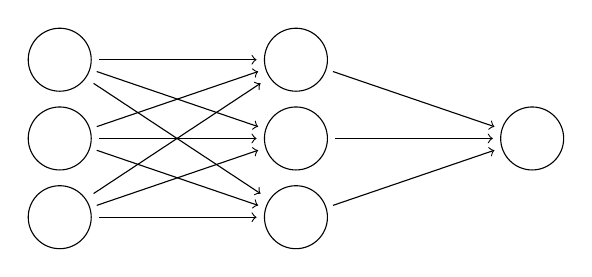
\begin{tikzpicture}
        
        \draw [] (0.5,1) circle [radius=0.4];
        \draw [] (0.5,0) circle [radius=0.4];
        \draw [] (0.5,-1) circle [radius=0.4];

        \draw [] (3.5,1) circle [radius=0.4];
        \draw [] (3.5,0) circle [radius=0.4];
        \draw [] (3.5,-1) circle [radius=0.4];

        \draw [] (6.5, 0) circle [radius=0.4];

        \draw[->] (1,1) -- (3,1);
        \draw[->] (0.97,0.85) -- (3.02,0.15);
        \draw[->] (0.93,0.7) -- (3.05,-0.7);

        \draw[->] (0.97,0.15) -- (3.02,0.85);
        \draw[->] (1,0) -- (3,0);
        \draw[->] (0.97,-0.15) -- (3.02,-0.85);

        \draw[->] (0.93,-0.7) -- (3.05,0.7);
        \draw[->] (0.97,-0.85) -- (3.02,-0.15);
        \draw[->] (1,-1) -- (3,-1);
        
        \draw[->] (3.97,0.85) -- (6.02,0.15);
        \draw[->] (4, 0) -- (6,0);
        \draw[->] (3.97, -0.85) -- (6.02,-0.15);

    \end{tikzpicture}
    \caption{The example neural network}
    \label{fig:backprop_one}
\end{figure}

%calculate output from network, error
First, the output from each layer is calculated as in section \ref{calculating_an_output}. The final output is then compared to a target output to calculate an error. This error is calculated with an error function, such as mean squared error (kilde).

[equation of error calculation]
$
Error = 
$


This error is used to calculate how much each weight should adjust.
[Equation for calculating ]
[Illustration of network with arrows backwards]

% calculate error backwards through all layers
Calculate error backward through all layers

[Illustration]

% calculate weightupdates
Calculate the weightupdate for each weight

[Illustration]

% update weights 
Update the weights

[Illustration]

% Short explaination for a deeper network
% The same process but more steps
For deeper networks

[Illustration]

\subsection{Dropout}
\label{dead-neurons}
% https://www.cs.toronto.edu/~hinton/absps/JMLRdropout.pdf
% 

Dropout is a technique used during training of a neural network. For a training sample, random units and all their connections are temporary dropped from the neural network \parencite{srivastava_dropout:_2014}. This means that the connections dropped will not be updated for this training sample. 

%Dropout implicitly splits the neural network into many thinned networks with shared weights. After training the 

\begin{figure}[H]
\centering
    \begin{subfigure}{1\textwidth} 
    \centering
        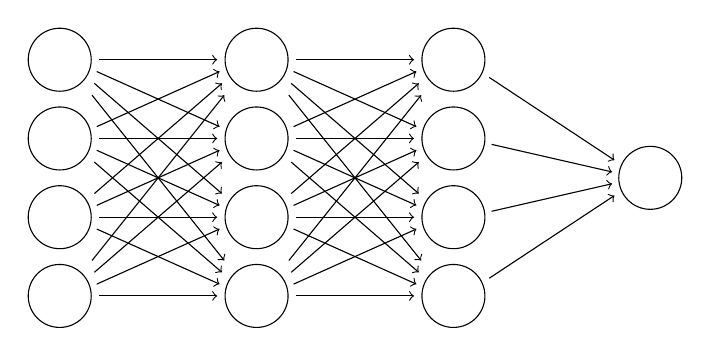
\begin{tikzpicture}

            \draw [] (-2.5,3) circle [radius=0.4];
            \draw [] (-2.5,2) circle [radius=0.4];
            \draw [] (-2.5,1) circle [radius=0.4];
            \draw [] (-2.5,0) circle [radius=0.4];

            \draw [] (0,3) circle [radius=0.4];
            \draw [] (0,2) circle [radius=0.4];
            \draw [] (0,1) circle [radius=0.4];
            \draw [] (0,0) circle [radius=0.4];

            \draw [] (2.5,3) circle [radius=0.4];
            \draw [] (2.5,2) circle [radius=0.4];
            \draw [] (2.5,1) circle [radius=0.4];
            \draw [] (2.5,0) circle [radius=0.4];
            
            \draw [] (5,1.5) circle [radius=0.4];
            
            
            \draw[->] (-2,3) -- (-0.5,3);
            \draw[->] (-2.03,2.85) -- (-0.47,2.15);
            \draw[->] (-2.06,2.7) -- (-0.44,1.30);
            \draw[->] (-2.09,2.55) -- (-0.41,0.45);
            
            \draw[->] (-2.03,2.15) -- (-0.47,2.85);
            \draw[->] (-2,2) -- (-0.5,2);
            \draw[->] (-2.03,1.85) -- (-0.47,1.15);
            \draw[->] (-2.06,1.70) -- (-0.44,0.30);
            
            \draw[->] (-2.06,1.3) -- (-0.44,2.7);
            \draw[->] (-2.03,1.15) -- (-0.47,1.85);
            \draw[->] (-2,1) -- (-0.5,1);
            \draw[->] (-2.03,0.85) -- (-0.47,0.15);
            
            \draw[->] (-2.09,0.45) -- (-0.41,2.55);
            \draw[->] (-2.06,0.30) -- (-0.44,1.7);
            \draw[->] (-2.03,0.15) -- (-0.47,0.85);
            \draw[->] (-2,0) -- (-0.5,0);
            
            
            \draw[->] (0.5,3) -- (2,3);
            \draw[->] (0.47,2.85) -- (2.03,2.15);
            \draw[->] (0.44,2.7) -- (2.06,1.30);
            \draw[->] (0.41,2.55) -- (2.09,0.45);
            
            \draw[->] (0.47,2.15) -- (2.03,2.85);
            \draw[->] (0.5,2) -- (2,2);
            \draw[->] (0.47,1.85) -- (2.03,1.15);
            \draw[->] (0.44,1.70) -- (2.06,0.30);
            
            \draw[->] (0.44,1.3) -- (2.06,2.7);
            \draw[->] (0.47,1.15) -- (2.03,1.85);
            \draw[->] (0.5,1) -- (2,1);
            \draw[->] (0.47,0.85) -- (2.03,0.15);
            
            \draw[->] (0.41,0.45) -- (2.09,2.55);
            \draw[->] (0.44,0.30) -- (2.06,1.7);
            \draw[->] (0.47,0.15) -- (2.03,0.85);
            \draw[->] (0.5,0) -- (2,0);
            
            
            \draw[->] (2.955,2.775) -- (4.545,1.725);
            \draw[->] (2.985,1.925) -- (4.515,1.575);
            \draw[->] (2.985,1.075) -- (4.515,1.425);
            \draw[->] (2.955,0.225) -- (4.545,1.275);
            
            
        \end{tikzpicture}
    \caption{}
    \label{fig:net_without_dropout}
    \end{subfigure}
    \begin{subfigure}{1\textwidth}
    \centering
        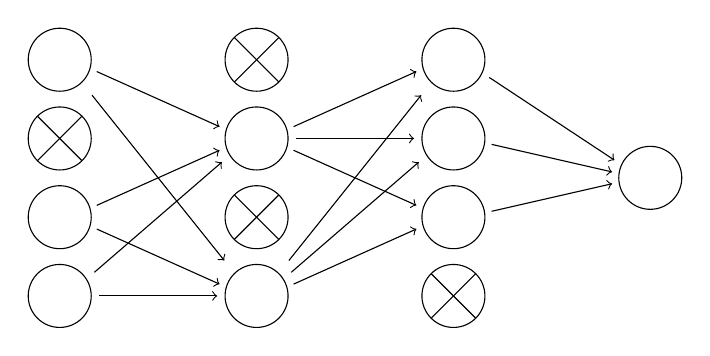
\begin{tikzpicture}
            \draw [] (-2.5,3) circle [radius=0.4];
            \draw [] (-2.5,2) circle [radius=0.4];
            \draw [] (-2.5,1) circle [radius=0.4];
            \draw [] (-2.5,0) circle [radius=0.4];

            \draw [] (0,3) circle [radius=0.4];
            \draw [] (0,2) circle [radius=0.4];
            \draw [] (0,1) circle [radius=0.4];
            \draw [] (0,0) circle [radius=0.4];

            \draw [] (2.5,3) circle [radius=0.4];
            \draw [] (2.5,2) circle [radius=0.4];
            \draw [] (2.5,1) circle [radius=0.4];
            \draw [] (2.5,0) circle [radius=0.4];
            
            \draw [] (5,1.5) circle [radius=0.4];
            
            \draw[-] (-2.78,2.28) -- (-2.22,1.72);
            \draw[-] (-2.78,1.72) -- (-2.22,2.28);
            
            \draw[-] (-0.28,3.28) -- (0.28,2.72);
            \draw[-] (-0.28,2.72) -- (0.28,3.28);
            
            \draw[-] (-0.28,1.28) -- (0.28,0.72);
            \draw[-] (-0.28,0.72) -- (0.28,1.28);
            
            \draw[-] (2.22,0.28) -- (2.78,-0.28);
            \draw[-] (2.22,-0.28) -- (2.78,0.28);
            
            
            \draw[->] (-2.03,2.85) -- (-0.47,2.15);
            \draw[->] (-2.09,2.55) -- (-0.41,0.45);
            
            \draw[->] (-2.03,1.15) -- (-0.47,1.85);
            \draw[->] (-2.03,0.85) -- (-0.47,0.15);
            
            \draw[->] (-2.06,0.30) -- (-0.44,1.7);
            \draw[->] (-2,0) -- (-0.5,0);
            
            
            \draw[->] (0.47,2.15) -- (2.03,2.85);
            \draw[->] (0.5,2) -- (2,2);
            \draw[->] (0.47,1.85) -- (2.03,1.15);
            
            \draw[->] (0.41,0.45) -- (2.09,2.55);
            \draw[->] (0.44,0.30) -- (2.06,1.7);
            \draw[->] (0.47,0.15) -- (2.03,0.85);
            
            
            \draw[->] (2.955,2.775) -- (4.545,1.725);
            \draw[->] (2.985,1.925) -- (4.515,1.575);
            \draw[->] (2.985,1.075) -- (4.515,1.425);
        \end{tikzpicture}
    \caption{}
    \label{fig:net_with_dropout}
    \end{subfigure}
\caption{Neural networks without (A) and with (B) dropout applied. The crossed circles are the dropped units.}
\label{fig:dropout_comparison}
\end{figure}

The purpose of dropout is to reduce the chance of overfitting a neural network. A neural network is overfitted when it is too closely related to the training samples, and not being as generalized as possible. An overfitted neural network will give good results if tested with the training data, but might fail on new data that the neural network has not seen before. In \cite{srivastava_dropout:_2014}, classifiers and neural networks trained with and without dropout applied is compared using standardized data sets. In every comparison, neural networks with dropout was ranked high, if not highest.

%illstration of overfitting


\section{Common problems}

\subsection{Vanishing gradient}
\label{vanishing-gradient}
\subsection{Exploding gradient}

\subsection{Dead neurons}

\section{Feedforward neural networks}
% 
Feedforward neural networks is also often referred to as deep feedforward networks or multilayer perceptrons (MLPs) are the most typical of deep learning models. The ultimate goal of feedforward neural networks is to approximate some function \textbf{f}, for example a task to classify (map) an input x to a specific class y. y = \textbf{f*(x)} in mathematical notation. The networks mapping is defined as y = \textbf{f(x,$\theta$)} where $\theta$ is learned in the way that \textbf{f} is approximated in the best way possible. \\ % HÅV
\cite{goodfellow_deep_2016}[p.~163] explains why networks such as these are called feedforward.
\begin{displayquote}[\cite{goodfellow_deep_2016}]
These models are called \textbf{feedforward} because information flows through the function being evaluated from \textbf{x}, through the intermediate computations used to define f, and finally to the output \textbf{y}. There are no \textbf{feedback} connections in which outputs of the model are fed back into itself.
\end{displayquote}



\subsection{Convolutional Networks}
% is feedforward with convolutional mathematical operations between some layers
% convolutional layers: conv_1d, 2d, explain kernels
% explaing pooling layers
% image recognition
% pros cons
% 
% TODO CITE LeCun 1989 ?!
Convolutional networks is also often referred to as convolutional neural networks or CNNs. CNNs are specialized for processing data that has a known typology. Examples includes images, which is an 2D-grid of pixels and say time series data. In this attempt to get some accurate classifications for handwritten mathematics we are both using images and sequential data. The reason that CNNs are actually called a CNN is because they use a convolution, which is a mathematical operation.
\begin{displayquote}[\cite{goodfellow_deep_2016}]
 \textit{Convolutional networks are simply neural networks that use convolution in place of general matrix multiplication in at least one of their layers.}
\end{displayquote}
To understand this further, the convolution operation needs to be explained. A convolution can be explained as an operation on two functions which has real-valued arguments.\\ 

% TRENGER VI EKSEMPEL? VELDIG LIKT GOODFELLIG
The example \cite{goodfellow_deep_2016} uses to explain a convolution is as follows; we are tracking the location of a spaceship with a laser. Our laser is feeding us a single output x(t), which reads the position of the spaceship at time t. Now if the laser is noisy we may read data that could be unrepresentative. Thus, we could need some sort of average function and in addition to averaging we would also like to specify that the most recent recordings are most important. This is solvable using weights, w(a) is our weighting function, where a is the age of a measurement.
\begin{figure}[H]
    \label{eqn:conv}
    \begin{equation}
    s(t) = \int x(a)w(t-a) da
    \end{equation}
    \caption{\cite{goodfellow_deep_2016}[p.~322] Example convolution which averages sensor readings and weights the most recent sensor readings. w(a) is the weighting function, x(t) is the position of the spaceship at time t. The result of this is a new function s, which gives us a smoothed estimate}
\end{figure}

\begin{figure}[H]
    \label{fig:conv_asterisk}
    \begin{equation}
        s(t) = (x*w)(t)
    \end{equation}
    \caption{Asterisk notation of a convolution.}
\end{figure}
% TRENGER VI EKSEMPEL? VELDIG LIKT GOOFELLOW
The first argument is called input, the second argument is often called kernel and the output of this is often called the \textbf{feature map}. In the example with lasers x would be our input and w would be the kernel. % Eksempel på feature map ?
\\
% Diskret notasjon
In a perfect world the laser would be able to provide real-time measurements, but that is not realistic. Often readings are discretized, that means that a new reading will arrive at a given interval, an example of this could be a new reading every second. This would eventually lead to t being an integer and since both x and w is dependent on t we end up with the discrete convolution. \parencite{goodfellow_deep_2016}
\begin{figure}[H]
    \label{fig:disc_conv}
    \begin{equation}
        s(t) = (x*w)(t) = \sum_{a=-\infty}^{\infty} x(a)w(t-a)
    \end{equation}
    \caption{\cite{goodfellow_deep_2016}[p.~323] definition on the discrete convolution.}
\end{figure}
For two-dimensional inputs, there is two-dimensional kernels, which is commutative:
\begin{figure}[H]
    \label{fig:disc_conv2d}
    \begin{equation}
        S(i,j) = (I*K)(i,j) = \sum_{m} \sum_{n} I(m,n)K(i-m,j-n)
    \end{equation}
    \begin{equation}
        S(i,j) = (K*I)(i,j) = \sum_{m} \sum_{n} I(i-m,j-n)K(m,n)
    \end{equation}
    \caption{\cite{goodfellow_deep_2016}[p.~323] the two dimensional kernel in both it's original form in addition to the version with the flipped kernel. The last version is a result of \textbf{flipping} the kernel relative to it's input.}
\end{figure}
% SJEKK OM VI TRENGER KOMMUTATIVE ALTERNATIVET. 
The actual function that usually exists in machine learning libraries is \textbf{cross-correlation}. \textbf{Cross-correlation} is the same as a convolution without flipping the kernel and it is often referred to as convolution.
\begin{figure}[H]
    \begin{equation}
        S(i,j) = (K*I)(i,j) = \sum_{m} \sum_{n} I(i+m,j+n)K(m,n)
    \end{equation}
    \label{fig:cross_corr}
    \caption{\cite{goodfellow_deep_2016}[p.~324] the \textbf{cross-correlation} function.}
\end{figure}
\textbf{Sparse interactions, connectivity or weights} is a result of making the kernel smaller than the input. Even if an image has many thousands of pixels it is possible to extract small crucial features using smaller kernel sizes.
\begin{figure}[H]
    \centering
    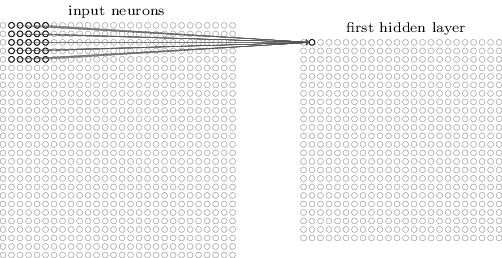
\includegraphics[width=\textwidth]{Assets/Chapter2_Theory/kernel_applied.png}
    \caption{This figure from \cite{nielsen_neural_2015} shows how a convolution layer works with a 5x5 kernel, also referred to as a filter or feature detector. In this example, our input is 28x28, if we apply a 5x5 kernel we will end up with 24x24 neurons in the hidden layer. Available from http://neuralnetworksanddeeplearning.com/images/tikz45.png, 23.04.2018}
    \label{fig:kernel_applied}
\end{figure}
%In summary the convolutional layer accepts a volume of size \textbf{$W_1$ x $H_1$ x $D_1$}. In addition to a volume, it needs to provide four \gls{hyperparameters}. These \gls{hyperparameters} are the number of filters \textbf{K}, their spartial extent \textbf{F}, the stride \textbf{S} and the ammount of zero padding \textbf{P}. 
A convolutional layer has typically three stages, the first is to do the convolutions as illustrated in \ref{fig:kernel_applied}, these are linear activations. When all the convolutions are done, they are passed through a nonlinear activation function. An example of a \gls{nonlinear} activation function is the sigmoid function \ref{eqn:sigmoid}. Furthermore this stage is often referred to as the \textbf{detector} stage.

\begin{equation}\label{eqn:sigmoid}
    \sigma(x) = \frac{1}{1+e^{-x}}
\end{equation}
The last stage of the a typical convolutional layer is when we apply a \textbf{pooling function}\parencite{zhou_computation_1988} to further modify the output. A \textbf{pooling function} is able to replace the output of a small area with a summary of the nearby outputs. There are multiple pooling functions, in our project and for our purpose we went with \textbf{max pooling}. The max pooling function uses a pooling unit which has a specified size, for example 2x2. The pooling unit in a max pooling function simply outputs the maximum activation of it's region(2x2), a max pooling function with a pooling unit region of 2x2 would turn 24x24 neurons to 12x12 neurons. \parencite{goodfellow_deep_2016} \parencite{nielsen_neural_2015}

\section{Recurrent neural networks}
% sequences
% time dimension
% pros cons
Recurrent neural networks, also often referred to as RNNs \parencite{rumelhart_learning_1986} are neural networks which can process sequential data. CNNs are sort of specialized on taking and analyzing grid like data, such as images or videos. RNNs on the other hand are more specialized on processing data that is sequential. The idea behind RNNs is to share parameters in different parts of a model. Sharing parameters makes it possible to use the model on data with variable length. \begin{displayquote}[\cite{goodfellow_deep_2016}]
 \textit{Such sharing is particularly important when a specific piece of information can occur at multiple positions within the sequence.}
\end{displayquote}
Furthermore an artificial neuron or computing unit is not only determined by it's activations in previous layers, it is now possible for an artificial neuron or computing unit to be determined by it's own activation earlier. \\ \parencite{goodfellow_deep_2016} \parencite{nielsen_neural_2015} \\\\
Data provided by the CROHME competitions is sequential ink coordinates as illustrated in listing \ref{lst:InkML_ex}. Thus, the principle of information sharing is quite significant in this projects case as well. % TODO sjekk om dette er bra eksempel. Kanskje bruk heller at skal man lære et språk må man lære alle regler for hver posisjon i en setning for eksempel, noe som gjør treningen og oppgaven veldig vanskelig.

\subsection{Long-short term memory}
Long-short term memory is often referred to as LSTM. Long-short term memory recurrent networks has something called "LSTM cells". L

\subsection{Gated Recurrent Unit}
Gated recurrent unit is often referred to as GRU.